\section{Software Quality Metrics}
Citat fra Troels: \textit{''Hvad kan man finde ud af om sit program, uden at køre det? Denne disciplin kaldes Static Analysis, og kan give feedback til programmøren, der er ligeså værdifuld som en faktisk test.''}\\

Statisk analyse kan bruges til: 

\begin{enumerate}
	\item Give \textit{quality measures}.
	\item Gennemtvinge \textit{code style and decipline}.
	\item Finde \textit{possible errors}.
\end{enumerate}

\subsection{Værktøjer} til formålet har vi nogle værktøjer.

\subsubsection{FxCop}
Statisk analyseværktøj, udviklet af Microsoft til Visual Studio. Lavet for at øge performance, sikkerhed og design.

\subsubsection{Compilers}
Compileren er et eksempel på et Statisk analyseværktøj. Alle moderne compilere viser advarseler og lignende for koden, nogle vigtige, andre not so much.

\subsection{Quantitative code analysis}
Aka: Software Metrics. Bruges til at beskrive: 

\begin{itemize}
	\item Lines of code per function/module.
	\item Cyclomatic complexity (se afsnit~\ref{sec:cyclomatic}).
	\item Microsoft Maintainability index.
\end{itemize}

\subsubsection{Maintainability}
Et index som beskriver hvor holdbar og effektiv ens kode er. Samt hvor let den er at vedligeholde. Indexet beregnes på følgende måde.

\subsubsection{Cyclomatic Complexity}\label{sec:cyclomatic}
Bruges til at beskrive kompleksiteten i et program. Det er et kvantitativt mål for antallet af lineære uafhængige vejen gemmet programmets source code.

\begin{figure}[H]
	\centering
	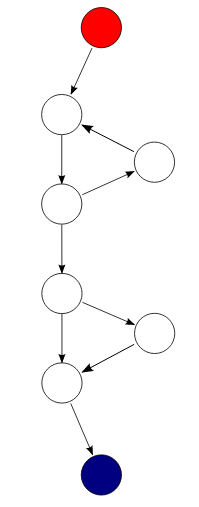
\includegraphics[width=0.8\linewidth]{figs/cyclomatic}
	\caption{Grafisk fremstiling af den cyclomatiske complexity i code listing~\ref{code:cyclomatic}.}
	\label{fig:cyclomatic}
\end{figure}

\begin{lstlisting}[caption=Kode for eksempel vist på figur~\ref{fig:cyclomatic}.,label=code:cyclomatic]
public void Method() {
	while(Condition1) 
		Action1();		
	if(Condition2) 
		Action2();		
	Action3();	
	return;
}
\end{lstlisting}

Når man har en graf som vist på figur~\ref{fig:cyclomatic}, er følgende udtryk gældende: 

\begin{align}
E &= NumberOfEdges\\
N &= NumberOfNodes\\
P &= NumberOfConnectionComponents
\end{align}

\vskip.3cm

Med disse termer kan M (antallet af \textit{decision points}) findes sådan her:

\begin{align}
M &= E-N+2P\\
M&= 9-8+2*1=3
\end{align}































